\documentclass[]{article}

\usepackage{amsmath}
\usepackage{graphicx}
\usepackage{amssymb}
\usepackage{esdiff}
\usepackage{hyperref}
\graphicspath{.}

%opening
\title{Double Pendulum: Theory}
\author{Ben Hoberman}

\begin{document}
	
\date{June 17, 2017 -- July 25, 2017}
\maketitle

\newcommand{\lagr}{\mathcal{L}}

\section{Introduction}
As it turns out, simulating a double pendulum is kind of complicated. Some research divulged that Lagrangian mechanics might give me an easier way to understand the behavior of this system, so after some research and an MIT online lecture (available \href{https://www.youtube.com/watch?v=zhk9xLjrmi4&t=3925s}{here}), here is my attempt at figuring out a double pendulum.

\section{Describing the System}
\begin{figure}[h!]
	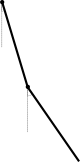
\includegraphics[height=5cm]{situation}
	\caption{A crude image of a double pendulum}
\end{figure}
$\theta_1$ represents angle between the anchored stick and the vertical, and $\theta_2$ represents the the angle between the free stick and the vertical. Both increase with counterclockwise rotation. The anchored stick has length $l_1$ and mass $m_1$, while the free stick has length $l_2$ and mass $m_2$.

In order to write the Lagrangian for this system, we need to choose a generalized coordinate system and express the system's kinetic and potential energies in terms of those coordinates. We will use $\theta_1$ and $\theta_2$ as our system's generalized coordinates.

The two sticks are the only elements of the system that account for its kinetic energy. All of the anchored stick's kinetic energy can be easily expressed as rotational kinetic energy, but the free stick will have a translational kinetic energy in addition to a rotational one, both about the stick's center.

In order to calculate the speed of the center of mass of the free stick, we must do some math. The cartesian coordinates of the centers of mass of the two sticks are as follows:
\begin{gather*}
x_1 = \frac{\ell_1}{2}\sin(\theta_1) \\
y_1 = -\frac{\ell_1}{2}\cos(\theta_1) \\
x_2 = \ell_1\sin(\theta_1) + \frac{\ell_2}{2}\sin(\theta_2) \\
y_2 = -\ell_1\cos(\theta_1) - \frac{\ell_2}{2}\cos(\theta_2)
\end{gather*}
In order to find the linear velocity, we can use the good old Pythagorean theorem to figure out that $v = \sqrt{\dot{x}^2 + \dot{y}^2}$, or, even more conveniently, that $v^2 = \dot{x}^2 + \dot{y}^2$ for the free stick stick. Let's do that:
\begin{gather*}
	v_2^2 = \dot{x_2}^2 + \dot{y_2}^2 = (\dot{\theta_1}\ell_1\cos(\theta_1) + \dot{\theta_2}\frac{\ell_2}{2}\cos(\theta_2))^2 + (\dot{\theta_1}\ell_1\sin(\theta_1) + \dot{\theta_2}\frac{\ell_2}{2}\sin(\theta_2))^2 \\
	= \dot{\theta_1}^2\ell_1^2 + \frac{\dot{\theta_2}^2\ell_2^2}{4} + \dot{\theta_1}\dot{\theta_2}\ell_1\ell_2\cos(\theta_1 - \theta_2) \\
	K_{\text{linear}} = \frac12m_2v_2^2 = \frac12m_2(\dot{\theta_1}^2\ell_1^2 + \frac{\dot{\theta_2}^2\ell_2^2}{4} + \dot{\theta_1}\dot{\theta_2}\ell_1\ell_2\cos(\theta_1 - \theta_2))
\end{gather*}
Because our selected independent coordinates describing the system are $\theta_1$ and $\theta_2$, describing the rotational kinetic energy of the system is much more simple. For each stick, $K_{rot} = \frac12 I \dot{\theta}^2$. The anchored stick has moment of intertia $\frac13m_1\ell_1^2$, and the free stick has moment of intertia $\frac{1}{12}m_2\ell_2^2$.
\begin{gather*}
	K_{\text{rotational}} = \frac16m_1\ell_1^2\dot{\theta_1}^2 + \frac{1}{24}m_2\ell_2^2\dot{\theta_2}^2
\end{gather*}

We can now find the total kinetic energy of the system:
\begin{gather*}
	K = K_{linear} + K_{rot} \\
	= \frac12m_2(\dot{\theta_1}^2\ell_1^2 + \frac{\dot{\theta_2}^2\ell_2^2}{4} + \dot{\theta_1}\dot{\theta_2}\ell_1\ell_2\cos(\theta_1 - \theta_2)) + \frac16m_1\ell_1^2\dot{\theta_1}^2 + \frac{1}{24}m_2\ell_2^2\dot{\theta_2}^2
\end{gather*}

In order to find the Lagrangian of the system, we must also describe the potential energy of the system at any given time. Gravitational potential energy accounts for the potential energy in this system, so let us describe the gravitational potential energy of the system with respect to the bottom position, where $\theta_1 = \theta_2 = 0$:
\begin{gather*}
	U_g = \sum mg\Delta h = m_1gy_1 + m_2gy_2 \\
	= -\frac{\ell_1m_1g}{2}\cos(\theta_1) - m_2g(\ell_1\cos(\theta_1) + \frac{\ell_2}{2}\cos(\theta_2)) \\
	= -g\cdot\frac{\ell_1m_1\cos(\theta_1) + 2m_2\ell_1\cos(\theta_1) + m_2\ell_2\cos(\theta_2)}{2} \\
	= -g\cdot\frac{(\ell_1m_1 + 2m_2\ell_1)\cos(\theta_1) + m_2\ell_2\cos(\theta_2)}{2}
\end{gather*}

Now that we have calculated the kinetic and potential energies of the system, we can calculate the Lagrangian, $\lagr = K - V$, where $K$ is the total kinetic energy and $V$ is the total potential energy:
\begin{gather*}
	\lagr = K - V = \frac12m_2[\dot{\theta_1}^2\ell_1^2 + \frac{\dot{\theta_2}^2\ell_2^2}{4} + \dot{\theta_1}\dot{\theta_2}\ell_1\ell_2\cos(\theta_1 - \theta_2)] + \frac16m_1\ell_1^2\dot{\theta_1}^2 + \frac{1}{24}m_2\ell_2^2\dot{\theta_2}^2 \\ + \frac{g}{2}[(\ell_1m_1 + 2m_2\ell_1)\cos(\theta_1) + m_2\ell_2\cos(\theta_2)]
\end{gather*}

With the Lagrangian, we can set up the Euler-Lagrange differential equation for each coordinate:
\begin{gather*}
	\diff{}{t}\frac{\partial \lagr}{\partial \dot{\theta_i}} = \frac{\partial \lagr}{\partial \theta_i} \\
	\frac{\partial \lagr}{\partial \dot{\theta_1}} = \frac{2m_1\dot{\theta_1}\ell_1^2 + 6m_2\ell_1^2\dot{\theta_1} + 3m_2\ell_1\ell_2\dot{\theta_2}\cos(\theta_1 - \theta_2)}{6} \\
	\diff{}{t}\frac{\partial \lagr}{\partial \dot{\theta_1}} =  \frac{2m_1\ddot{\theta_1}\ell_1^2 + 6m_2\ell_1^2\ddot{\theta_1} + 3m_2\ell_1\ell_2\ddot{\theta_2}\cos(\theta_1 - \theta_2) - 3m_2\ell_1\ell_2\dot{\theta_2}\sin(\theta_1 - \theta_2)(\dot{\theta_1} - \dot{\theta_2})}{6} \\
	\frac{\partial \lagr}{\partial \theta_1} = -\frac{m_2\ell_1\ell_2\dot{\theta_1}\dot{\theta_2}\sin(\theta_1 - \theta_2)}{2} - g\cdot\frac{(\ell_1m_1 + 2m_2\ell_1)\sin(\theta_1)}{2} \\
\end{gather*}

\begin{gather*}
	\frac{\partial \lagr}{\partial \dot{\theta_2}} = \frac{2m_2\ell_2^2\dot{\theta_2} + 3m_2\ell_1\ell_2\dot{\theta_1}\cos(\theta_1 - \theta_2)}{6} \\
	\diff{}{t}\frac{\partial \lagr}{\partial \dot{\theta_2}} = \frac{2m_2\ell_2^2\ddot{\theta_2} + 3m_2\ell_1\ell_2\ddot{\theta_1}\cos(\theta_1 - \theta_2) - 3m_2\ell_1\ell_2\dot{\theta_1}\sin(\theta_1 - \theta_2)(\dot{\theta_1} - \dot{\theta_2})}{6} \\
	\frac{\partial \lagr}{\partial \theta_2} = \frac{m_2\ell_1\ell_2\dot{\theta_1}\dot{\theta_2}\sin(\theta_1 - \theta_2)}{2} - g\cdot\frac{m_2\ell_2\sin(\theta_2)}{2}
\end{gather*}

We can now solve these two differential equations for $\ddot{\theta_1}$ and $\ddot{\theta_2}$, which together will be used in our simulation.

\begin{gather*}
	(2m_1\ell_1^2 + 6m_2\ell_1^2)\ddot{\theta_1} + 3m_2\ell_1\ell_2\cos(\theta_1 - \theta_2)\ddot{\theta_2} \\
	= 3 m_2\ell_1\ell_2\dot{\theta_2}\sin(\theta_1 - \theta_2)(\dot{\theta_1} - \dot{\theta_2}) - 3m_2\ell_1\ell_2\dot{\theta_1}\dot{\theta_2}\sin(\theta_1 - \theta_2) - 3g(\ell_1m_1 + 2m_2\ell_1)\sin(\theta_1) \\
	3m_2\ell_1\ell_2\cos(\theta_1 - \theta_2)\ddot{\theta_1} + 2m_2\ell_2^2\ddot{\theta_2} \\ 
	= 3m_2\ell_1\ell_2\dot{\theta_1}\sin(\theta_1 - \theta_2)(\dot{\theta_1} - \dot{\theta_2}) + 3m_2\ell_1\ell_2\dot{\theta_1}\dot{\theta_2}\sin(\theta_1 - \theta_2) - 3g m_2\ell_2\sin(\theta_2) \\
	\text{We will find the two $\ddot{\theta}$'s using a matrix solution} \\
	\vec{b} = \begin{bmatrix}
		3 m_2\ell_1\ell_2\dot{\theta_2}\sin(\theta_1 - \theta_2)(\dot{\theta_1} - \dot{\theta_2}) - 3m_2\ell_1\ell_2\dot{\theta_1}\dot{\theta_2}\sin(\theta_1 - \theta_2) - 3g(\ell_1m_1 + 2m_2\ell_1)\sin(\theta_1) \\
		3m_2\ell_1\ell_2\dot{\theta_1}\sin(\theta_1 - \theta_2)(\dot{\theta_1} - \dot{\theta_2}) + 3m_2\ell_1\ell_2\dot{\theta_1}\dot{\theta_2}\sin(\theta_1 - \theta_2) - 3g m_2\ell_2\sin(\theta_2)
	\end{bmatrix} \\
	\boldsymbol{A} = \begin{bmatrix}
		2m_1\ell_1^2 + 6m_2\ell_1^2 & 3m_2\ell_1\ell_2\cos(\theta_1 - \theta_2) \\
		3m_2\ell_1\ell_2\cos(\theta_1 - \theta_2) & 2m_2\ell_2^2
	\end{bmatrix} \\
	\vec{\ddot{\theta}} = \boldsymbol{A}^{-1}\vec{b}
\end{gather*}

We now have a pair of second order differential equations that describes the motion of the system. Using the Runge-Kutta method (aka RK4), we can approximate solutions for $\theta_1$ and $\theta_2$ over some time interval. First, let us redefine this system as a single vector function:

\begin{gather*}
	\theta = 
	\begin{bmatrix}
		\theta_1 \\
		\theta_2
	\end{bmatrix} \text{, }
	\dot{\theta} = 
	\begin{bmatrix}
		\dot{\theta_1} \\
		\dot{\theta_2}
	\end{bmatrix} \text{, and }
	\ddot{\theta} =
	\begin{bmatrix}
		\ddot{\theta_1} \\
		\ddot{\theta_2}
	\end{bmatrix} \\
	\ddot{\theta}(\theta, \dot{\theta}) = \boldsymbol{A}^{-1}\vec{b}\text{, according to $\boldsymbol{A}(\theta, \dot{\theta})$ and $\vec{b}(\theta, \dot{\theta})$ above}
\end{gather*}

Now we will set up the RK4 method for this system.

\begin{gather*}
	\text{Let } z = \dot{\theta}(\theta, \dot{\theta}) = \diff{\theta}{t} \text{, so } \diff{z}{t} = \ddot{\theta} \\
	z = \dot{\theta} \\
	\dot{z} = \ddot{\theta}(\theta, \dot{\theta}) \\
	\theta_{new} = \theta + \frac{h}{6}(k_0 + 2k_1 + 2k_2 + k_3) \\
	\dot{\theta}_{new} = \dot{\theta} + \frac{h}{6}(l_0 + 2\ell_1 + 2l_2 + l_3) \\
	\text{Let our step be $h$, and $k$ and $l$ are as follows:}\\
	k_0 = hz = h\dot{\theta}_0 \\
	l_0 = h\dot{z} = h\ddot{\theta}_0 \\
	k_1 = hz(\theta_0 + \frac{k_0}{2}, \dot{\theta}_0 + \frac{l_0}{2}) = h\cdot(\dot{\theta}_0 + \frac{l_0}{2}) \\
	\ell_1 = h\dot{z}(\theta_0 + \frac{k_0}{2}, \dot{\theta}_0 + \frac{l_0}{2}) = h\cdot\ddot{\theta}(\theta_0 + \frac{k_0}{2}, \dot{\theta}_0 + \frac{l_0}{2}) \\
	k_2 = hz(\theta_0 + \frac{k_1}{2}, \dot{\theta}_0 + \frac{\ell_1}{2}) = h\cdot(\dot{\theta}_0 + \frac{\ell_1}{2}) \\
	l_2 = h\dot{z}(\theta_0 + \frac{k_1}{2}, \dot{\theta}_0 + \frac{\ell_1}{2}) = h\cdot\ddot{\theta}(\theta_0 + \frac{k_1}{2}, \dot{\theta}_0 + \frac{\ell_1}{2}) \\
	k_3 = hz(\theta_0 + k_2, \dot{\theta}_0 + l_2) = h\cdot(\dot{\theta}_0 + l_2) \\
	l_3 = h\dot{z}(\theta_0 + k_2, \dot{\theta}_0 + l_2) = h\cdot\ddot{\theta}(\theta_0 + k_2, \dot{\theta}_0 + l_2)
\end{gather*}

Implementing this in code will get us our simulation. Hopefully.

\end{document}
